%Chap 3 pag 24
\definecolor{Pink}{RGB}{255,0,131}
\definecolor{DarkRed}{RGB}{128,0,0}

\begin{frame}{Ejemplo: Ensamblaje robótico}
\begin{figure}
    \centering
    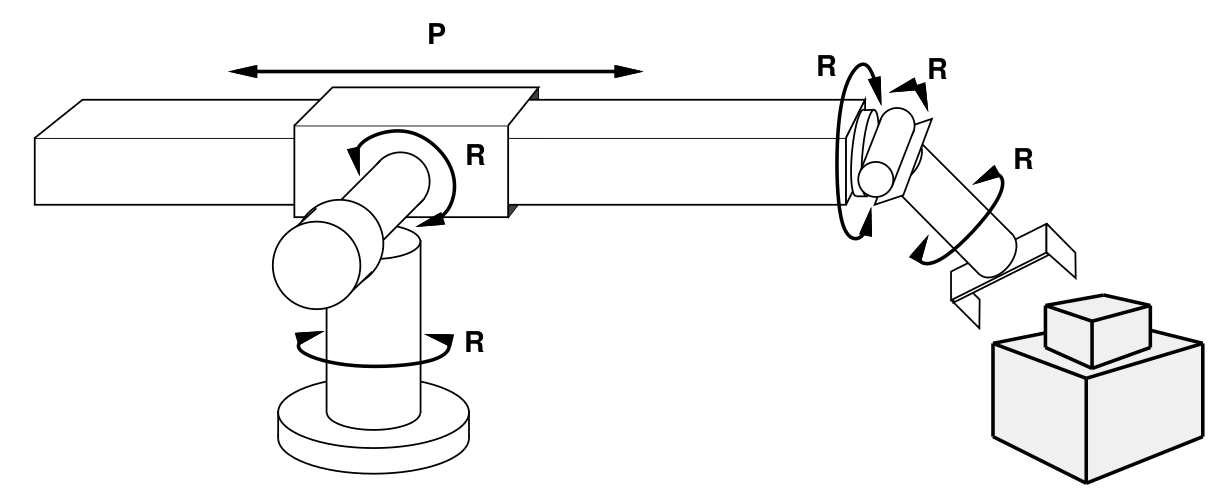
\includegraphics[scale=0.23]{24_chap3_pag24.png}
\end{figure}
\begin{flushleft}
    \textcolor{Pink}{¿Estados?}: Coordenadas, en valores reales, de los ángulos de unión de las partes del objeto a ensamblar.\\
    \textcolor{Pink}{¿Acciones?}: Movimientos continuos de las articulaciones del
    robot.\\
    \textcolor{Pink}{¿Estado de Objetivo?}: Montaje completo,
    \textcolor{DarkRed}{¡sin robot incluido!}\\
    \textcolor{Pink}{¿Costo de ruta?}: Tiempo de ejecución.
\end{flushleft}
\end{frame}
